
\chapter{Trace Analysis} 
\label{sec:trace}

We study two sets of real-world storage traces collected from large-scale
storage server environments and characterize their update patterns.  Motivated
by the fact that enterprises are considering erasure coding as an alternative
to RAID for fault-tolerant storage \cite{raid_alternatives}, we choose these
traces to represent the workloads of enterprise storage clusters and study the
applicability of erasure coding to such workloads.  We want to answer three
questions: (1) \textit{What is the average size of each update?} (2)
\textit{How common do data updates happen?} (3) \textit{Are updates focused on
some particular chunks?}  
%To this end, we identify the lessons learned from our analysis that guide our
%update design in erasure-coded storage. 

%Our work adopts a write-many-read-many (WMRM) semantics on files. While this
%is contrary to the write-once-read-many (WORM) using in many distributed file
%systems nowadays, we justify the needs for data update support by analysing
%real-world traces collected in research and academic institutes.

\section{Trace Description}

\subsection{MSR Cambridge traces.} We use the public block-level
I/O traces of a storage cluster released by Microsoft Research Cambridge
\cite{narayanan08}. The traces are captured %below the file system cache 
on 36 volumes of 179 disks located in 13 servers.  They are composed
of I/O requests, each specifying the timestamp, the server name, the disk
number, the read/write type, the starting logical block address, 
the number of bytes transferred, and the response time.  The whole
traces span a one-week period starting from 5PM GMT on 22nd February 2007, and
account for the workloads in various kinds of deployment including user home
directories, project directories, source control, and media.  Here, we choose
10 of the 36 volumes for our analysis.  Each of the chosen volumes contains
800,000 to 4,000,000 write requests. 

%Here, we only summarize the analysis results for the 10 volumes that are
%chosen for evaluation.  In our technical report [CITE], we present a full
%summary of analysis for all 36 volumes.

\subsection{Harvard NFS traces.}  We also use a set of NFS traces
(\texttt{DEAS03}) released by Harvard \cite{ellard04}.  The traces capture NFS
requests and responses of a NetApp file server 
%that serves home directories for Harvard's Division of Engineering and
%Applied Sciences, 
that contains a mix of workloads including email, research, and development.
The whole traces cover a 41-day period from 29th January 2003 to 10th March
2003.  Each NFS request in the traces contains the timestamp, source and
destination IP addresses, and the RPC function. 
%the transport protocol, the NFS RPC protocol version and direction, the RPC
%XID field and the RPC function. 
Depending on the RPC function, the request may contain optional fields such as
file handler, file offset and length.  While the traces describe the
workloads of a single NFS server, they have also been used in trace-driven
analysis for clustered storage systems \cite{abd05,hendricks06}.

%Unlike that in a block I/O trace, each NFS request in the trace is
%accompanied with a file handler, thus we are able to map individual requests
%to files. We make use of this information to evaluate the accuracy of our
%reserve space allocation algorithm in \S\ref{sec:design}. We apply
%similar treatment as the MSR Cambridge trace to merge adjacent sequential
%requests. 

% Compress caption spacing
%\setlength\abovecaptionskip{6pt minus 2pt}
%\setlength\belowcaptionskip{-8pt minus 1pt}
\section{Key Observations}

%Through analysing data update behaviour of the 36 MSR Cambridge traces and 41
%days of Harvard NFS trace, we make the following observations that can be use
%to drive our work.
%We study the traces and characterize the following update behaviors. 

\subsection{Updates are small.}  We study the update size, i.e., the number of
bytes accessed by each update.  Figure~\ref{fig:msr_dist} shows the average
update size ranges of the MSR Cambridge traces.  We see that the updates are
generally small in size. Although different traces show different
update size compositions, all updates occurring in the traces are smaller than
512KB. Among the 10 traces, eight of them have more than $60\%$ of updates
smaller than 4KB. Similarly, the Harvard NFS traces comprise small updates,
with average size of only 10.58KB, as shown in Table~\ref{table:harvard}.

% Compress caption spacing
%\setlength\abovecaptionskip{6pt minus 2pt}
\begin{figure}[t]
    \centering
    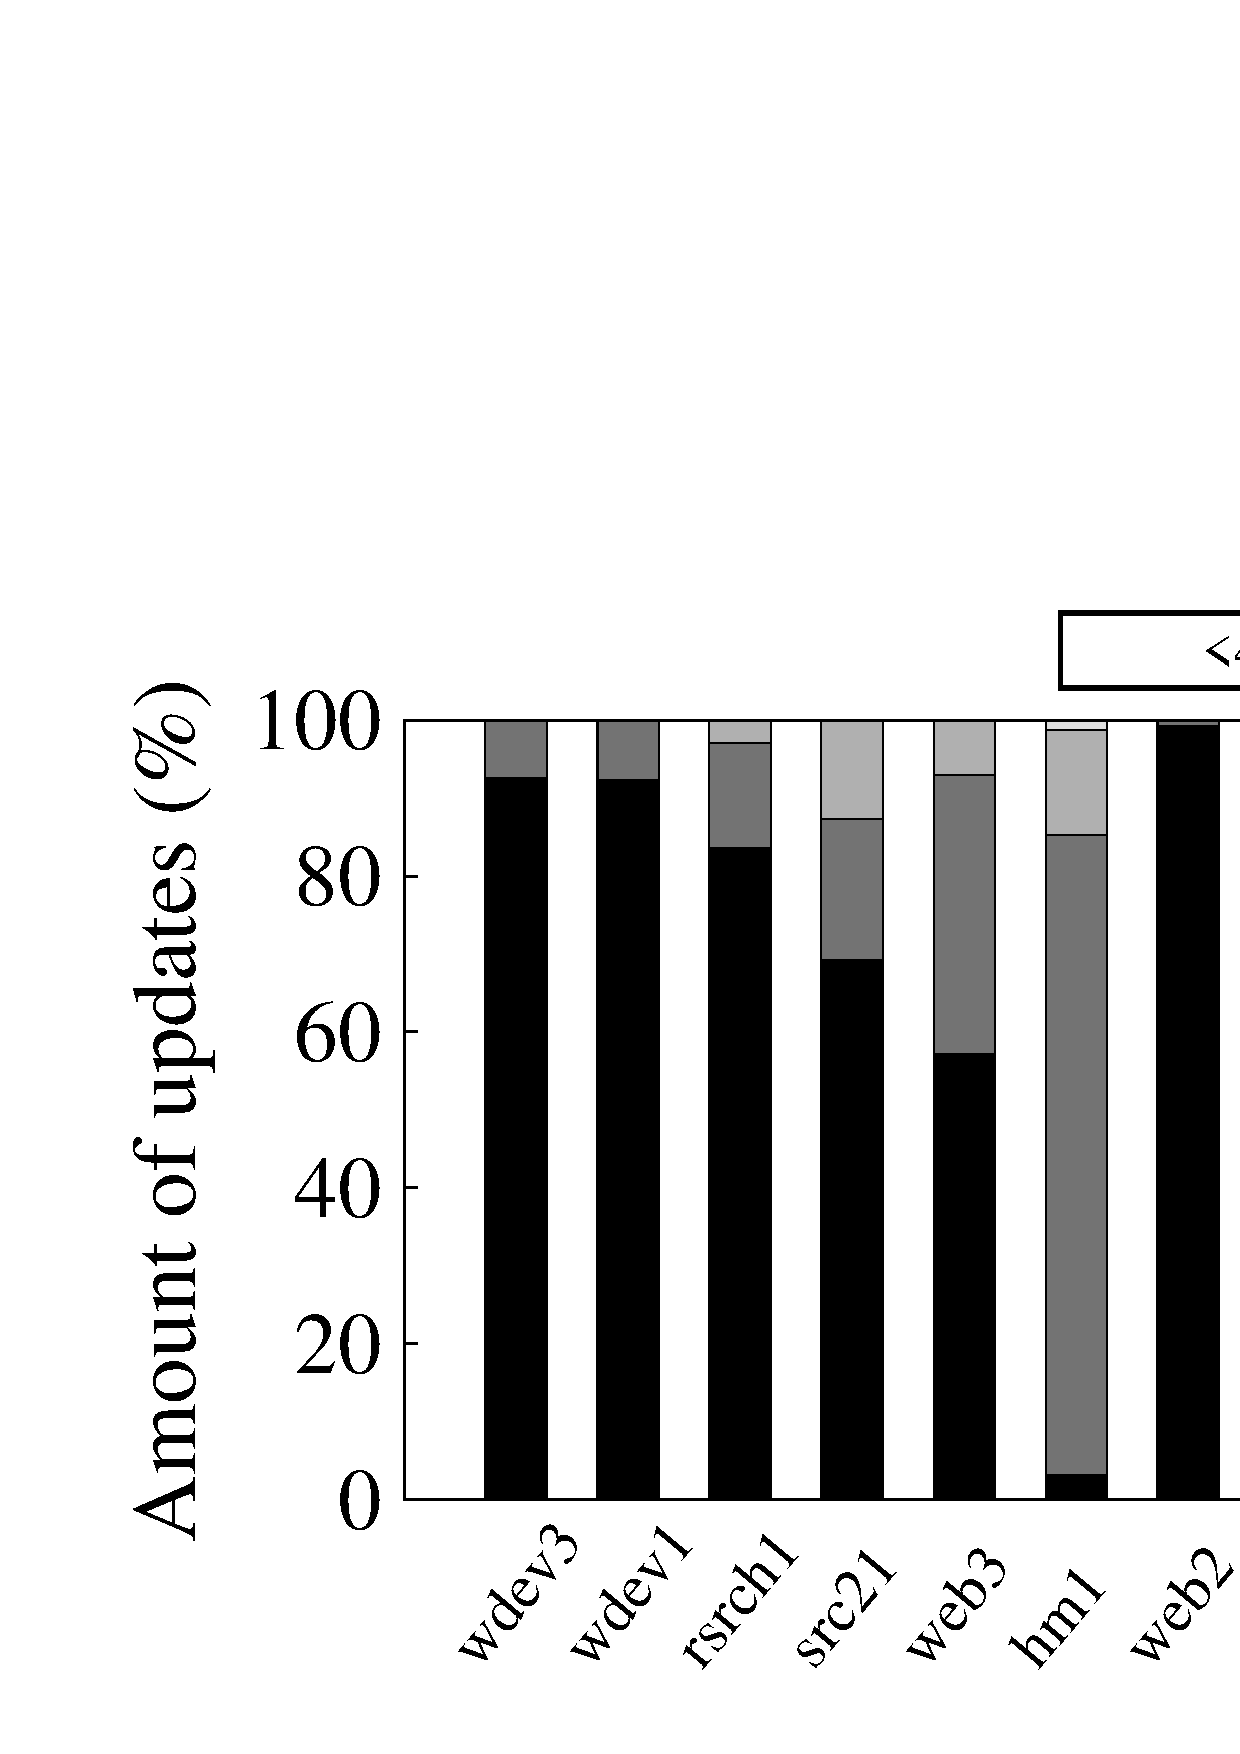
\includegraphics[width=0.9\linewidth]{charts/msr_dist/eps/msr_dist}
    \vspace{-3pt}
    \caption{Distribution of update size in MSR Cambridge traces.}
    \label{fig:msr_dist}
    \vspace{-6pt}
\end{figure}

\begin{table}[t] \footnotesize
  \centering
    \begin{tabular}{rl}
    \toprule
    No. of Writes & 172702071 \\
    WSS (GB) & 174.73 \\
%    Write Size (GB) & 1734.11 \\
    Updated WSS (\%) & 68.39 \\
    Update Writes (\%) & 91.56 \\
    No. of Accessed Files & 2039724 \\
    Updated Files (\%) & 12.10 \\
    Avg. Update Size Per Request (KB) & 10.58 \\
    \bottomrule
    \end{tabular}%
  \caption{Properties of Harvard \texttt{DEAS03} NFS traces.}
  \label{table:harvard}%
  \vspace{-2pt}
\end{table}%

\setlength{\tabcolsep}{3pt}
\begin{table}[!t]  \footnotesize
\centering
    \begin{tabular}{C{0.71cm}C{1.9cm}C{1cm}C{0.7cm}C{1.1cm}C{1.3cm}}
    \toprule
           Volume    & Workload \newline Type        & \hfill No. of \newline \hfill Writes & \hfill WSS \newline \hfill (GB) 
           & Updated \newline WSS(\%) & Update \newline Writes(\%) \\
    \midrule
         \raggedright src22   & \raggedright Source control  & \hfill 805955        & \hfill 20.17    & 99.57            &  99.68 \\
         \raggedright mds0    & \raggedright Media server      & \hfill 1067061       & \hfill 3.09     & 29.27            &  95.77 \\
         \raggedright rsrch0  & \raggedright Research        & \hfill 1300030       & \hfill 0.36     & 69.53            &  97.41 \\
         \raggedright usr0    & \raggedright Home directory       & \hfill 1333406       & \hfill 2.44     & 42.54            &  96.08 \\
         \raggedright web0    & \raggedright Web/SQL server    & \hfill 1423458       & \hfill 7.26     & 37.25            &  96.23 \\
         \raggedright ts0     & \raggedright Terminal server   & \hfill 1485042       & \hfill 0.91     & 49.84            &  95.65 \\
         \raggedright stg0    & \raggedright Web staging     & \hfill 1722478       & \hfill 6.31     & 21.04            &  97.82 \\
         \raggedright hm0     & \raggedright HW monitor      & \hfill 2575568       & \hfill 2.31     & 73.16            &  93.21 \\
         \raggedright prn1    & \raggedright Print server      & \hfill 2769610       & \hfill 80.9     & 18.55            &  73.43 \\
         \raggedright proj0   & \raggedright Project directory    & \hfill 3697143       & \hfill 3.16     & 56.67            &  98.89 \\
    \bottomrule
    \end{tabular}%
    \vspace*{3pt}\\
    %\small{* selected for evaluation}
	\caption{Properties of MSR Cambridge traces: (1) number of writes
		shows the total number of write requests; (2) working set size refers to
		the size of unique data accessed in the trace; 
		(3) percentage of updated working set
		size refers to the fraction of data in the working set that is updated
		at least once; and (4) percentage of update writes refers to the
		fraction of writes that update existing data.}
\label{table:msr}
%\vspace{6pt}
\end{table}


\subsection{Updates are common.} Unsurprisingly, updates are common in both
storage traces.  We analyze the write requests in the traces and classify them
into two types: {\em first-write}, i.e., the address is first accessed, and
{\em update}, i.e., the address is re-accessed.  Table~\ref{table:harvard}
shows the results of the Harvard NFS traces.  Among nearly $173$~million
write requests, more than $91\%$ of them are updates.  Table~\ref{table:msr}
shows the results of the MSR Cambridge traces. All the volumes show more than
$90\%$ of updates among all write requests, except for the print server volume
\texttt{prn1}. We see limited relationship between the working set size (WSS)
and the intensity of writes.  For example, the project volume \texttt{proj0}
has a small WSS, but it has much more writes than the source control volume
\texttt{src22} that has a large WSS.
%Also, $12.10\%$ of the files in the Harvard trace are updated at least once.

\subsection{Update coverage varies.} Although data updates are common in all
traces, the coverage of updates varies. %from trace to trace.
We measure the update coverage by studying the fraction of WSS that is updated
at least once throughout the trace period. For example, from the MSR Cambridge
traces in Table~\ref{table:msr}, the \texttt{src22} trace shows a $99.57\%$ of
updated WSS, while updates in the \texttt{mds0} trace only cover $29.27\%$ of
WSS. In other words, updates in the \texttt{src22} trace span across a large
number of locations in the working set, while updates in the \texttt{mds0}
trace are focused on a smaller set of locations.  The variation in update
coverage implies the need of a dynamic mechanism to improve update efficiency.

%\subsection{Lessons Learned}

%\paragraph{Summary.}
%The above analysis shows that there are workloads in which the majority of
%writes are small updates. Also, the variation in update coverage implies the
%need of a dynamic mechanism to improve update efficiency.
%caching alone may not be sufficient to achieve a good update performance.
%Therefore, our aim is to devise a mechanism that provides update efficiency. 

% Reset caption spacing
%\setlength\abovecaptionskip{10pt}
%\setlength\belowcaptionskip{0pt}
%%%%%%%%%%%%%
% OLD DRAFT %
%%%%%%%%%%%%%

%If we put the trace into CodFS's context with
%RDP coding, 16M segments and $(n,k)=(6,4)$, on average each data fragment is
%modified more than \red{$400$} times, except for the \texttt{src2\_2} trace
%where the number of writes is small but has a large working set size. For
%log-structured file systems, updates to the same fragment are scattered
%throughout the disk. This fragmentation results in degraded performance in
%sequential read and recovery.  We back this claim by the experiment results in
%\S\ref{eval:trace}.

%\subsection {Update Locality}
%
%We ask the following questions related to update behaviour.
%\begin{itemize}
%    \item How common blocks are updated after they are first written?
%    \item What is the time difference between an update and the previous access
%         to the block? (we want to show that the caching approach by CAROM is
%         infeasible if the workload has a long tail)
%     \item How large is each update? (we want to show that simple reconstruction
%          write - our baseline approach is not good enough)
%  \end{itemize}
%
